\chapter{Introducción}
\label{chap:introduccion}

\section{El problema y su dificultad}

\subsection{Dos problemas en una misma pregunta}

¿Puede un sistema aprender a ordenar acciones fuera de muestra y convertir después ese orden en una
cartera útil? La pregunta parece única, pero contiene dos problemas. Ordenar exige que las acciones
con mayor puntuación obtengan, en promedio, mejores retornos futuros que las de menor puntuación.
Invertir exige además elegir cuántas comprar, cuánto asignar, cuándo vender y cuánto efectivo
mantener. Una señal puede resolver el primer problema y fracasar en el segundo.

Esa separación organiza todo el trabajo. El modelo se selecciona únicamente por su capacidad de
ordenación transversal; las reglas de cartera se estudian después, con la señal ya congelada. Así,
una mejora económica no puede reescribirse retrospectivamente como mejora predictiva.

A esa separación se añade una segunda decisión, tomada antes de calcular nada: los datos de 2025 y
2026 se apartaron desde el principio, y ninguna elección del trabajo ---ni el modelo, ni sus
parámetros, ni las reglas de cartera--- pudo mirarlos. El motivo es que un sistema elegido con los
mismos datos con los que después se juzga siempre parece mejor de lo que es, y ninguna corrección
estadística devuelve del todo esa inocencia. Reservar un tramo desde el inicio es la única forma de
llegar al final con una medición que la búsqueda no haya podido contaminar. Tiene un precio, y hay
que declararlo desde ya: ese tramo es corto y, con un horizonte de doce meses, deja pocas
observaciones completas, así que sirve para comprobar si el sistema se sostiene, no para estimar con
precisión cuánto.

\subsection{Por qué es difícil}

La selección cuantitativa de acciones combina tres dificultades. Primero, la información disponible
cambia con el tiempo: usar hoy la composición actual de un índice o un dato fundamental antes de su
publicación produce una ventaja inexistente. Segundo, probar muchas configuraciones aumenta la
probabilidad de elegir ruido. Tercero, el resultado observado depende de una cadena de decisiones
posteriores al modelo. Evaluar solo la rentabilidad final no permite saber en qué eslabón apareció la
mejora o el fallo.

El sistema estudiado afronta esas dificultades con un panel \textit{point-in-time}, cohortes
cerradas y una única ruta experimental. Cinco agentes especializados ---calidad, valor, crecimiento, tendencia y riesgo---
producen cada uno su propia ordenación, y un meta-agente aprende a combinarlas con información que
ya estaba cerrada en cada fecha. La selección
secuencial modifica una variable cada vez y conserva únicamente cambios respaldados por Rank-IC
robusto. Después se calculan atribución, robustez, carteras y perfiles como evidencia informativa.

El segundo objetivo parte, además, de un listón competitivo muy alto. El \textit{SPIVA U.S.
Scorecard Year-End 2025} compara fondos estadounidenses de gran capitalización con el S\&P 500 y
muestra que la mayoría queda por debajo del índice en todos los horizontes publicados
(Figura~\ref{fig:spiva-horizontes}): a veinte años, el 92,89\,\% no lo supera.

\begin{figure}[htbp]
  \centering
  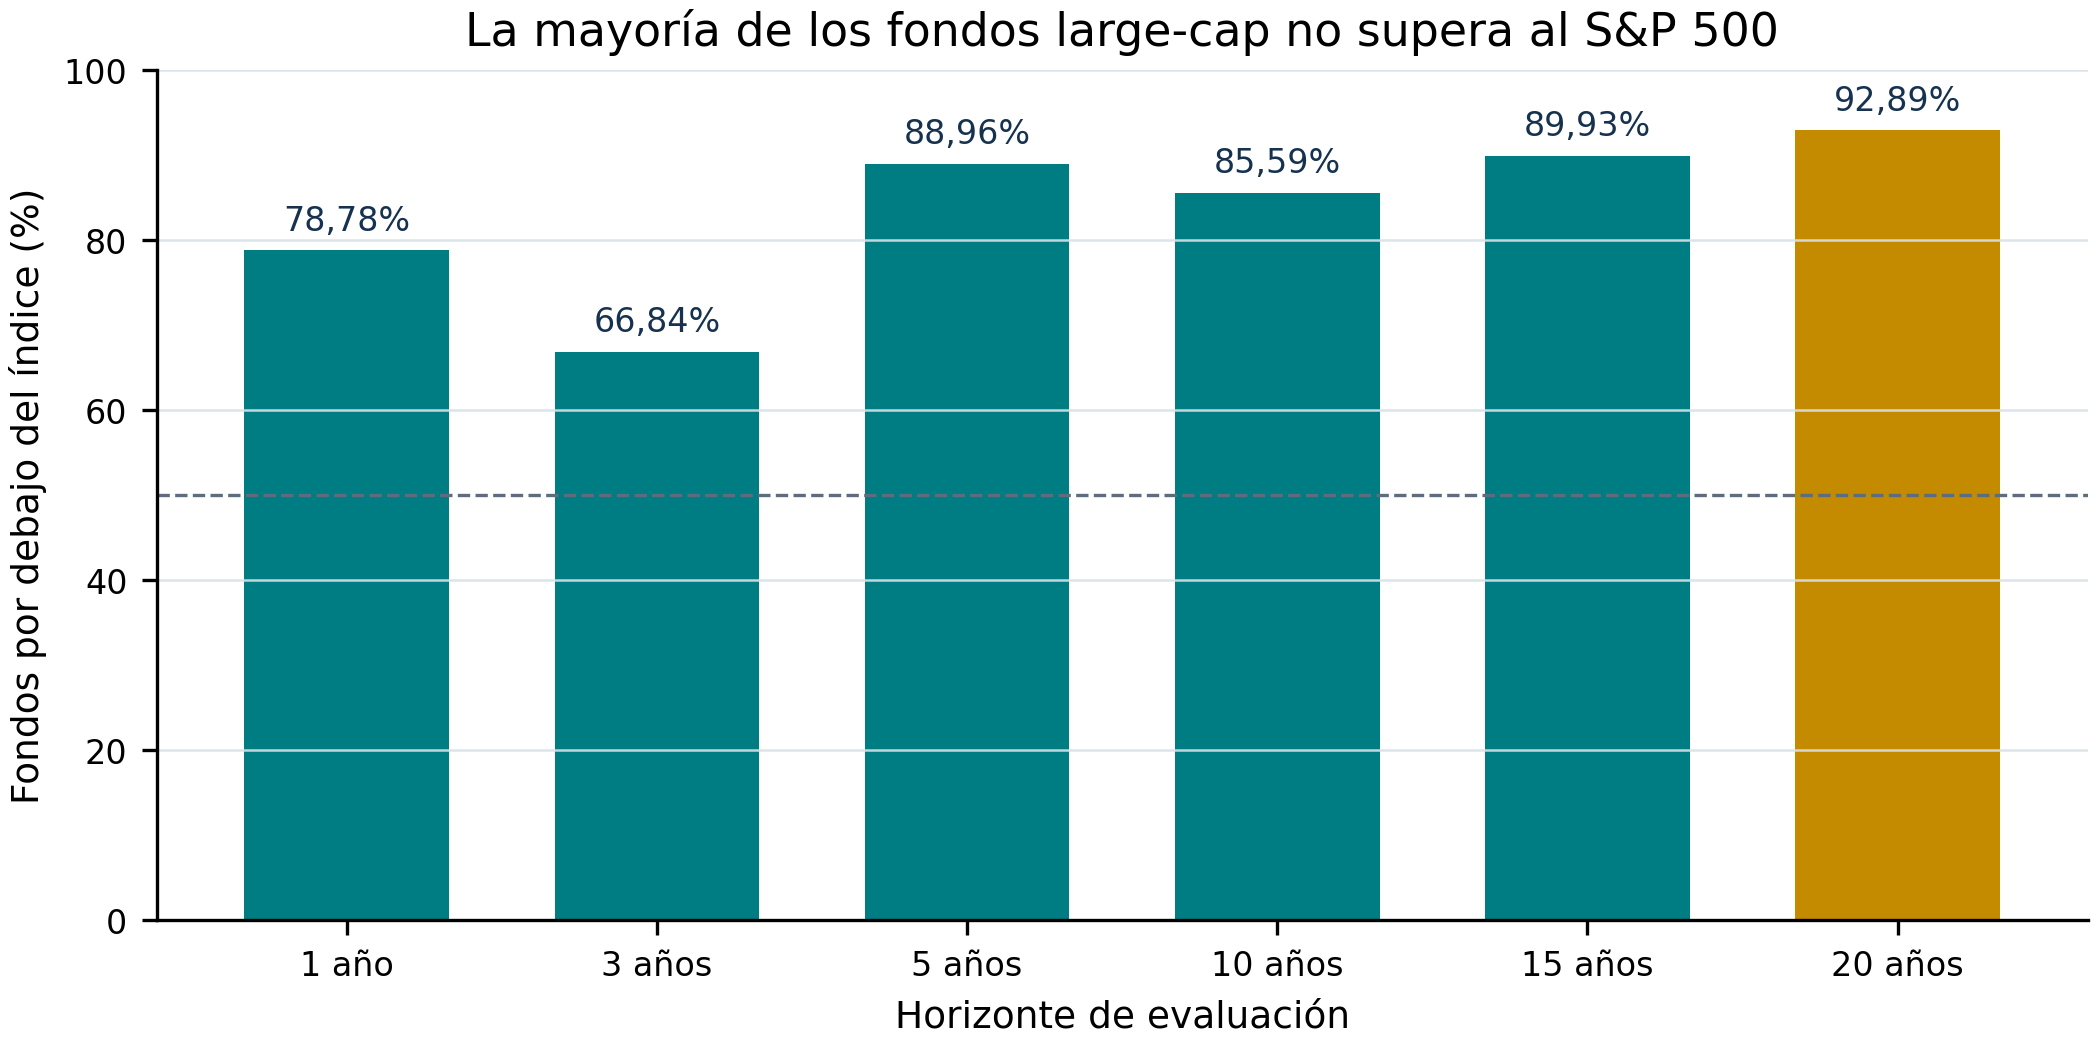
\includegraphics[width=0.94\textwidth]{figures/f01_spiva_horizontes.png}
  \caption{Fondos estadounidenses de gran capitalización que quedan por debajo del S\&P 500 a
  distintos horizontes. Fuente: S\&P Dow Jones Indices, \textit{SPIVA U.S. Scorecard Year-End
  2025}, Report 1a, rentabilidad absoluta; datos a 31 de diciembre de 2025.}
  \label{fig:spiva-horizontes}
\end{figure}

Esa persistencia no es una casualidad estadística: tiene una explicación aritmética.

\subsection{Por qué batir al índice es un juego de suma cero}
\label{sec:suma-cero-intro}

El argumento lo formuló Sharpe (1991) y es aritmético, no empírico: el mercado es la suma de quienes
lo componen, de modo que el conjunto de los gestores activos posee, por construcción, la cartera de
mercado. Antes de costes, el rendimiento medio ponderado de la gestión activa es exactamente el del
índice; para que alguien lo supere, otro debe quedarse por debajo en la misma medida. Es un juego de
\textbf{suma cero antes de costes}, y como operar cuesta, pasa a ser de \textbf{suma negativa
después}. No hay ninguna versión de este problema en la que todos los participantes ganen.

El argumento es exacto sobre el conjunto de los participantes, no sobre cada uno: no dice que sea
imposible batir al índice, sino que hacerlo exige que otro no lo consiga. Eso no vuelve inalcanzable
el objetivo económico, pero sí eleva el estándar de evidencia. No basta con encontrar una cartera
que funcionó en el periodo observado: hay que separar la capacidad de ordenar de la capacidad de
cobrar esa ventaja, descontar costes y comprobar qué sucede fuera de la ventana en la que se
eligieron las reglas.

\section{Dos objetivos}

\textbf{Objetivo 1. ¿Aprende el sistema a ordenar acciones?} Determinar si aprende una ordenación
transversal con capacidad predictiva fuera de muestra, y si esa capacidad resiste cambios de régimen
y controles contra azar, fuga temporal y factores conocidos. Es una afirmación sobre el modelo, se
mide con Rank-IC y se responde contra un listón absoluto: o existe una ordenación con Rank-IC
positivo fuera de muestra, o no existe. Este objetivo no presupone que el meta-agente deba superar a
todos los especialistas: esa comparación forma parte del resultado.

\textbf{Objetivo 2. ¿Puede cobrarse esa ordenación frente al mercado?} Comprobar si el orden
aprendido se traduce en una cartera que supere al índice una vez descontados los costes. A diferencia
del primero, es una afirmación sobre un mercado competitivo y de suma cero, y por tanto se responde
contra un listón relativo: superarlo significa ganarle la posición a otro participante en un juego
donde la mayoría pierde. Ninguna cantidad de Rank-IC lo garantiza por sí sola.

La respuesta a ese segundo objetivo depende de algo que este trabajo no esperaba encontrar en el
centro del argumento, y de ahí que se enuncie en dos mitades. \textbf{(2a)} Con la señal ya
congelada, ¿generan las reglas de construcción de cartera diferencias materiales en el resultado
económico? \textbf{(2b)} ¿Conserva la cartera elegida ese resultado en la era reservada? La primera
mitad puede sostenerse con toda la rejilla de alternativas; la segunda queda limitada por el reducido
número de cohortes reservadas. La respuesta, adelantada aquí, es que la misma señal produce
resultados de signo opuesto según cómo se construya la cartera: el segundo objetivo no puede
responderse sin declarar con cuál se midió.

\section{Aportación y recorrido del documento}

La aportación no consiste en presentar una cartera como recomendación de inversión. Consiste en un
procedimiento auditable para separar aprendizaje predictivo e implementación económica, junto con
un caso empírico completo. El trabajo muestra qué aprendió el sistema, qué especialista concentra la
información, qué contrastes supera, qué reglas de cartera mueven el resultado y qué cambia cuando la
misma señal se evalúa en una ventana que no intervino en ninguna decisión.

El documento sigue ese mismo orden. Los capítulos 2 a 5 preparan la respuesta ---la literatura, los
datos disponibles, el sistema y el protocolo que lo decide---; el 6 contesta a la primera pregunta y
el 7 a la segunda; el 8 delimita hasta dónde llega la evidencia y el 9 la resume.


